\subsection{Kết quả thử nghiệm cải thiện RUL}
\label{sec:rul-improvement-results}

Đợt thử nghiệm hoàn tất ngày 27/09/2026 chưa tìm được phương án đáp ứng đầy đủ
tiêu chí cải thiện đã chốt. Window 30 được chọn trong cả năm vòng ngoài.
Ở bước chỉnh tham số, vòng ngoài 1 và 3 chọn learning rate 0,03, 400 vòng
boosting, 31 lá tối đa, 10 mẫu tối thiểu tại lá và L2 bằng 0,01. Ba vòng còn
lại giữ cấu hình gốc. Không vòng nào chọn phương án tăng trọng số RUL thấp.
Vì vậy, bảng ablation đánh giá cả quy trình lựa chọn; không phải năm lần
đánh giá một cấu hình mới cố định.

\begin{table}[H]
\centering\small
\caption{Outer evaluation trên cùng 100 train engines và 17.731 khóa từ cycle 30. MAE tính bằng cycles; tỷ lệ thời gian báo sớm tính bằng phần trăm.}
\label{tab:rul-improvement-outer}
\begin{tabular}{L{4.3cm}rrrr}
\toprule
Phương án & MAE toàn bộ & MAE RUL $\leq30$ & Trễ/bỏ lỡ & Báo sớm (\%)\\
\midrule
Baseline & 20,2143 & 3,6676 & 49/100 & 1,2933\\
Sau chọn window & 20,2143 & 3,6676 & 49/100 & 1,2933\\
Sau chỉnh tham số & 20,2459 & 3,6730 & 53/100 & 1,2580\\
Sau chọn trọng số & 20,2459 & 3,6730 & 53/100 & 1,2580\\
\bottomrule
\end{tabular}
\end{table}

MAE RUL thấp tăng 0,0054 cycles, với paired bootstrap CI 95\%
$[-0{,}0506;0{,}0639]$. Chênh lệch MAE toàn bộ là 0,0315 cycles,
CI $[-0{,}1112;0{,}1737]$. Hai khoảng đều chứa 0, nên không có bằng chứng
về giảm sai số trong phép so sánh này. Tỷ lệ cảnh báo trễ hoặc bỏ lỡ tăng
4 điểm phần trăm, CI $[1;8]$ điểm phần trăm. Tỷ lệ thời gian báo sớm giảm
0,0353 điểm phần trăm, CI $[-0{,}1320;0{,}0627]$. Các khoảng được tính trên
predictions đã lưu; không bao gồm biến thiên nếu lặp lại toàn bộ huấn luyện.

RMSE toàn trajectory giảm nhẹ từ 33,6359 xuống 33,6160 cycles; NASA score
giảm từ $1{,}8850\times10^8$ xuống $1{,}8129\times10^8$. Những mức giảm này
không bù cho việc các tiêu chí chính chưa đạt. NASA score là tổng trên nhiều
window và phạt lỗi bất đối xứng, nên không so trực tiếp tổng này với score
trên 100 điểm cuối của test.

\begin{figure}[H]
\centering
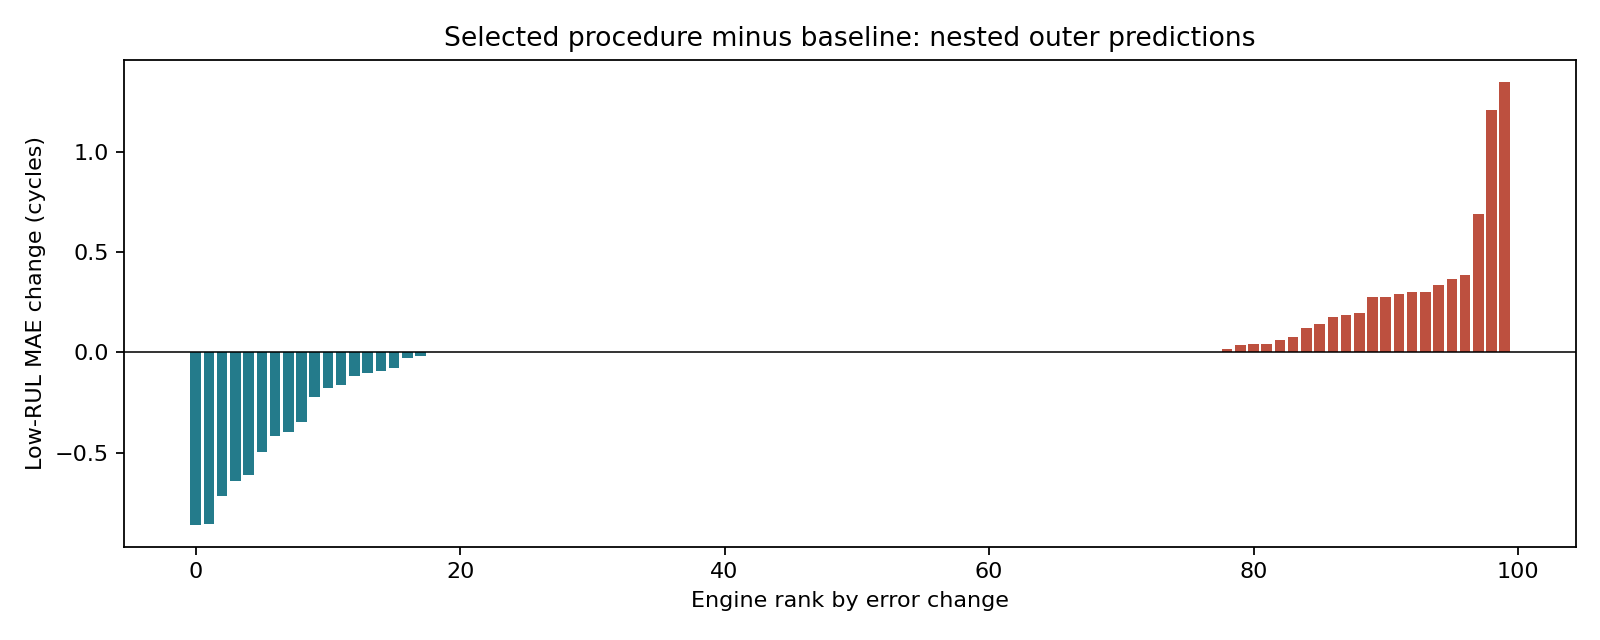
\includegraphics[width=0.97\textwidth]{../outputs/experiments/rul_improvement/20260927_full/figures/engine_error_delta.png}
\caption{Chênh lệch MAE RUL thấp của từng engine: quy trình chọn model trừ baseline. Giá trị âm biểu thị giảm sai số. Engine được sắp theo chênh lệch, không theo ID.}
\label{fig:rul-improvement-delta}
\end{figure}

\begin{figure}[H]
\centering
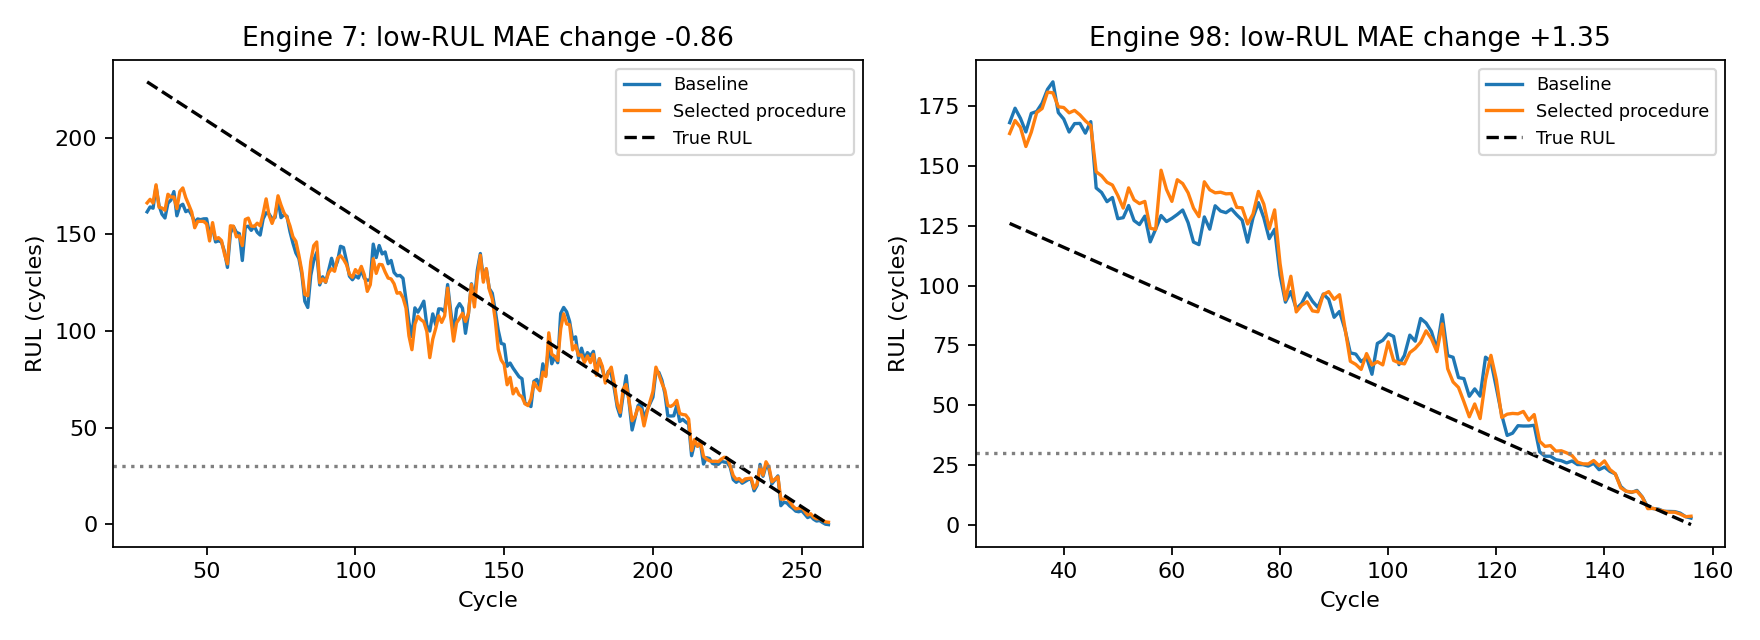
\includegraphics[width=0.99\textwidth]{../outputs/experiments/rul_improvement/20260927_full/figures/trajectory_examples.png}
\caption{Hai trường hợp có chênh lệch MAE RUL thấp nhỏ nhất và lớn nhất trong outer evaluation. Đây là ví dụ được chọn sau đánh giá để minh họa cả cải thiện và suy giảm.}
\label{fig:rul-improvement-trajectories}
\end{figure}

Engine 7 có MAE RUL thấp giảm từ 4,1811 xuống 3,3209 cycles, trong khi engine
98 tăng từ 3,9296 lên 5,2803 cycles. Cải thiện trên một engine không đủ để
kết luận cho toàn bộ dữ liệu. Cả hai phương án vẫn phát cảnh báo trên đủ
100 engines. Tuy nhiên, trung vị lead time giảm từ 30 xuống 29 cycles;
lead time nhỏ nhất vẫn là 19. Có cảnh báo ở mọi engine vì thế không bảo đảm
cảnh báo ở hoặc trước mốc nghiên cứu 30 cycles.

\begin{figure}[H]
\centering
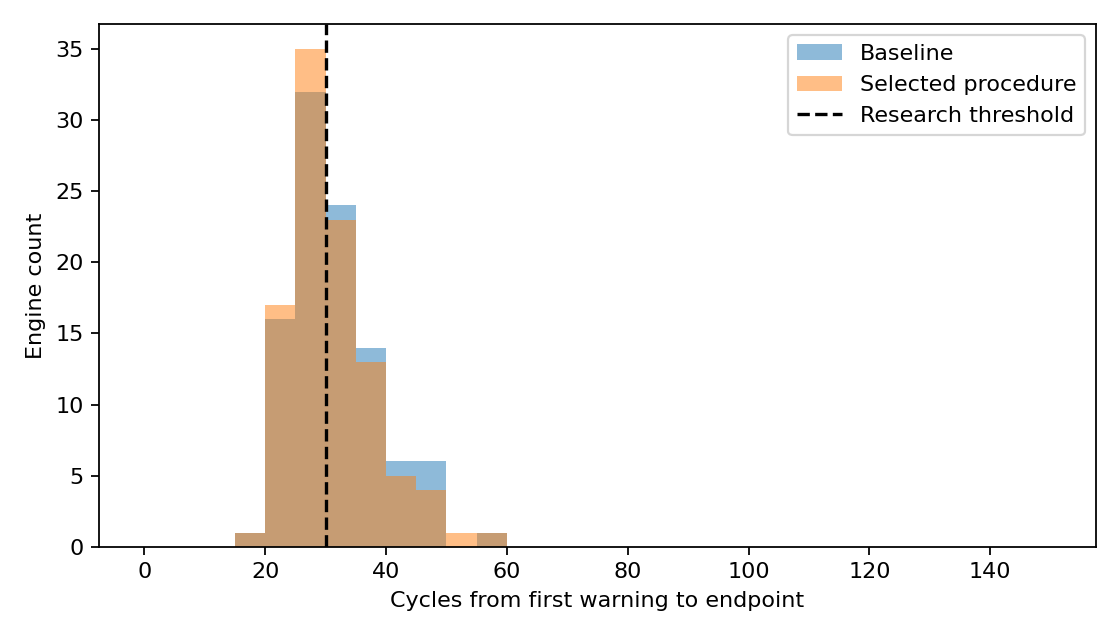
\includegraphics[width=0.82\textwidth]{../outputs/experiments/rul_improvement/20260927_full/figures/lead_time_comparison.png}
\caption{Phân phối lead time từ cảnh báo đầu tiên đến endpoint trên outer predictions. Đường đứt biểu thị mốc nghiên cứu 30 cycles.}
\label{fig:rul-improvement-lead-time}
\end{figure}

\subsubsection{Những đánh đổi quan sát được khi chọn cấu hình}

Không đáp ứng toàn bộ tiêu chí không có nghĩa mọi cấu hình đều không giảm
được sai số. Bảng~\ref{tab:rul-improvement-tradeoff} trình bày ba ví dụ từ
inner 3-fold trên toàn train, dùng ở bước chọn cấu hình cuối. Đây là kết quả
phục vụ lựa chọn, không phải đánh giá ngoài độc lập của từng cấu hình.

\begin{table}[H]
\centering\small
\caption{Ví dụ đánh đổi trong inner CV trên toàn train. Các dòng dùng cùng engine và cycle; không so số này trực tiếp với bảng outer evaluation.}
\label{tab:rul-improvement-tradeoff}
\begin{tabular}{L{4.3cm}rrrr}
\toprule
Ứng viên & MAE toàn bộ & MAE RUL $\leq30$ & Trễ/bỏ lỡ & Báo sớm (\%)\\
\midrule
Baseline & 20,3613 & 3,6148 & 50/100 & 1,2175\\
\texttt{hgb\_08} & 20,6846 & 3,2625 & 49/100 & 1,0177\\
Ưu tiên RUL thấp cao & 20,4072 & 3,3901 & 47/100 & 1,3752\\
\bottomrule
\end{tabular}
\end{table}

Ứng viên \texttt{hgb\_08} giảm MAE RUL thấp khoảng 9,75\%, nhưng tăng MAE
toàn bộ khoảng 0,3233 cycles. Phương án ưu tiên cao giảm sai số RUL thấp và
số cảnh báo trễ, nhưng tăng MAE toàn bộ và tỷ lệ thời gian báo sớm. Quy tắc
đã chốt không cho phép tăng các chỉ số kiểm soát, nên hai phương án không
được chọn. Nếu thay đổi mức đánh đổi chấp nhận được, cần công bố đó là một
đợt nghiên cứu tiếp theo; không sửa tiêu chí rồi coi kết quả hiện tại là
xác nhận độc lập cho tiêu chí mới.

\subsubsection{Cấu hình cuối và đánh giá test}

Inner CV trên toàn train chọn lại baseline: window 30, learning rate 0,05,
200 vòng boosting, 31 lá tối đa, 20 mẫu tối thiểu tại lá, L2 bằng 0 và trọng
số đồng đều trong mỗi engine. Model cuối được fit lại và ghi 100 test
predictions trước khi ghép nhãn NASA. Predictions khớp baseline, nên kết quả
test giữ nguyên như Bảng~\ref{tab:rul-improvement-test}.

\begin{table}[H]
\centering\small
\caption{Test endpoint evaluation: một prediction tại cycle cuối của mỗi engine. Nhóm RUL thật không quá 30 gồm 25 engines.}
\label{tab:rul-improvement-test}
\begin{tabular}{L{4.3cm}rrr}
\toprule
Model & MAE toàn bộ & RMSE & MAE RUL $\leq30$\\
\midrule
Baseline & 15,3490 & 20,5413 & 4,3830\\
Cấu hình được chọn cuối & 15,3490 & 20,5413 & 4,3830\\
\bottomrule
\end{tabular}
\end{table}

Đợt chạy lưu 511 fit cache riêng, tái sử dụng các fit trùng và có thêm một
lần fit model cuối. Kiểm tra xác nhận 100 engines được đánh giá ngoài, cùng
17.731 khóa cho bốn stage, engine separation trong 511 fit records, paired CI
tính lại khớp và predictions của model đã lưu khớp artifact. Baseline ban đầu
không bị thay đổi. Thực nghiệm vì vậy cung cấp một kết quả âm theo tiêu chí
đã chốt, đồng thời chỉ ra rõ những đánh đổi có thể nghiên cứu tiếp.
